\documentclass{article}
\usepackage{graphicx} % Required for inserting images
\usepackage{amsmath}
\usepackage{mathalfa}
\usepackage{blindtext}
\usepackage[letterpaper, portrait, margin=0.75in]{geometry}
\usepackage{amssymb}
\usepackage{epsf, subfigure, verbatim, epsfig}
\usepackage{fancyhdr}
\usepackage{calc}
\usepackage{ifthen}
\usepackage{layout}
\usepackage{fancybox}
\usepackage{eurosym}
\usepackage{tabularx}
\usepackage{xspace}
\usepackage{dsfont,mathrsfs}
\usepackage{amssymb}
\usepackage{theorem}
\usepackage{multicol}
\usepackage{float}
\usepackage{tikz}
\usepackage{pgfplots}
\pgfplotsset{compat=1.18}

\title{Homework 8 \\ \large MATH 476}
\author{Ahad Jiva}
\date{May 29, 2025}

\begin{document}

\maketitle

\section*{Exercise 85}
\begin{flushleft}
    Show that the price of a European put option on a non-dividend paying stock with strike price $K$ and expiry $T$ is 
    \begin{center}
        $p=Ke^{-rT}N(-d_2)-S_0N(-d_1)$.
    \end{center}
\underbar{Proof:} We will prove this using put-call parity. Recall that put-call parity states
\begin{center}
    $c + Ke^{-rT} = p + S_0$.
\end{center}
We also know that $c = S_0N(d_1) - Ke^{-rT}N(d_2)$. Plugging in this value of $c$ into the formula for put-call parity and isolating $p$, we get
\begin{center}
    $S_0N(d_1) - Ke^{-rT}N(d_2) + Ke^{-rT} = p + S_0$ \\
    $p = S_0N(d_1) - Ke^{-rT}N(d_2)+Ke^{-rT} - S_0$ \\
    $p = S_0 (N(d_1) - 1) + Ke^{-rT}(1-N(d_2))$ \\
    $p = S_0(-N(-d_1)) + Ke^{-rT}(N(-d_2))$ \\
    $p = Ke^{-rT}N(-d_2) - S_0N(-d_1)$
\end{center}
as desired. $\square$
\end{flushleft}

\section*{Exercise 99}
\begin{flushleft}
    Consider a stock that pays no dividends, has a volatility of 30\% per annum, and provides an expected return of 15\% per annum with continous compounding. The initial stock price is \$100. Use Monte Carlo simulation to simulate the stock price during one week periods for one year. \\
    Using the Monte Carlo method three separate times, we get
    \begin{center}
        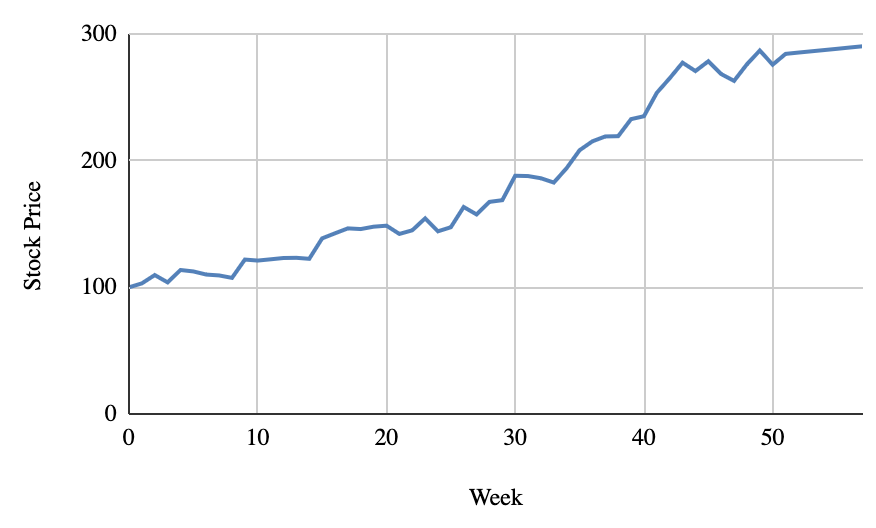
\includegraphics[width=0.5\textwidth]{mc1.png}
        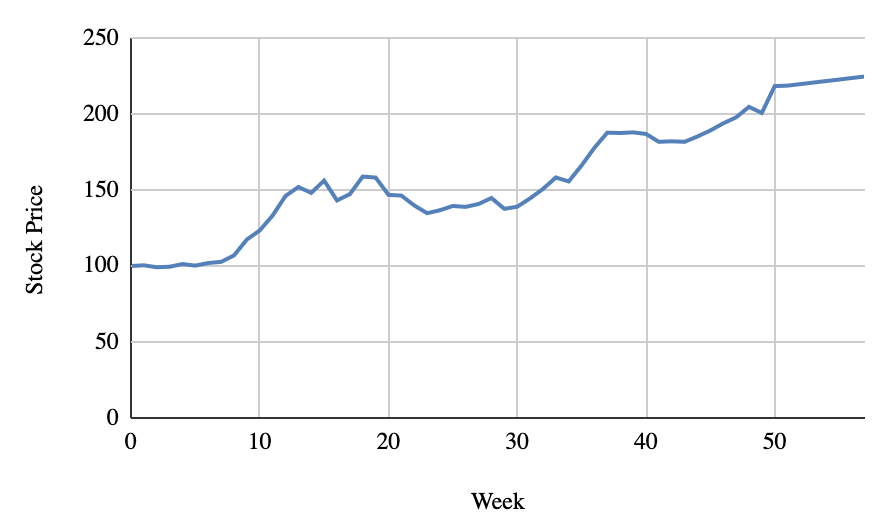
\includegraphics[width=0.5\textwidth]{mc2.png}
        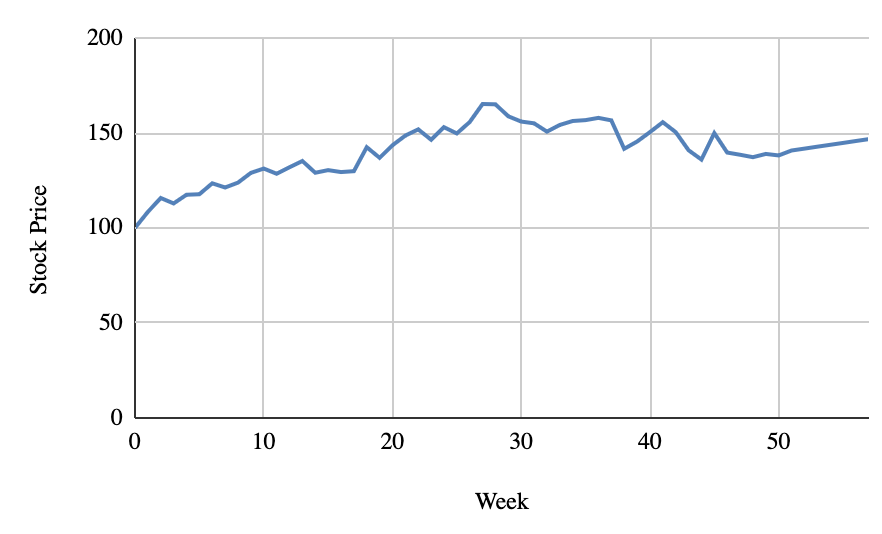
\includegraphics[width=0.5\textwidth]{mc3.png}
    \end{center}
    With each simulation, we get different results due to the random nature of the way we sample the normal distribution. The first simulation, the stock price nearly touches \$300, in the second, it barely cracks \$220, and in the last it fails to finish the year above \$150.
\end{flushleft}
\section*{Exercise 100}
\begin{flushleft}
    The Ito process for the stock price is $\Delta S = \mu S \Delta t + \sigma S \epsilon \sqrt{\Delta t}$. Explain the difference between this model and each of the following.
    \begin{enumerate}
        \item $\Delta S = \mu \Delta t + \sigma \epsilon \sqrt{\Delta t}$. This model is indifferent to the stock price, meaning that with this model, a stock worth \$5 and a stock worth \$50000 would move by the same amounts, which is not accurate.
        \item $\Delta S = \mu S \Delta t + \sigma \epsilon \sqrt{\Delta t}$. Although this model will take into account the stock's initial price, it does not adjust the drift term over time, meaning that in the long run, stock price changes will not vary. For example, if a stock starts at \$5, this model may work for some time, but as the stock increases to many multiples of 5, the model will become less and less accurate.
        \item $\Delta S = \mu \Delta t + \sigma S \epsilon \sqrt{\Delta t}$. With this model, $\Delta S$ will always be constant (plus or minus a "chaos" term). This would not be accurate in the long term as the stock price changes.
    \end{enumerate}
    It is also important to note that all three of these models violate the no-arbitrage principle. Consider a stock worth \$0. Then all three of these models imply that $\Delta S$ will be a nonzero value, which violates the no-arbitrage principle.
\end{flushleft}

\end{document}
